\section{Proposed methodology}
According to the discussion above, although there are existed work about the exemplar-based image inpainting algorithm \cite{cvpr03,tip04}. But previous attach a little too much calculation work to do when inpainting, it will result in long time to wait. Based on the previous work about exemplar-based image inpainting algorithm, we proposed a new evaluation criteria about the priority of each patch, which costs much less time than previous work and get good inpainted result.
\subsection{Two key observations}
\noindent \emph{A. Basic process unit size is important}

When select the exemplar region to inpaint the target region, the basic process unit size is important. The size of basic will effect the final result. Previous work has applied pixel as the basic unit\cite{iccv99}, the result will result in smoothing and blurring. It's easy to understand because small unit size ignore the connection between the each part of the image. Hence, we should not choose too small size of basic process unit. 

However, when the size of basic unit is too large, the target region inpainting will lead in to much difference. The large region of the mask region will get too much influence by the known region. That is to say, the target region will result in strange margin and line. So we should not choose too large basic process unit.

In our experiment, we test different unit size and compare them. Due to the difference of the number of calculation, process speed of each unit size is much different. Consider several factors, this algorithm present good results when the basic process size is $3*3$ or $5*5$.  Smaller size will result in smoothing and blurring, and larger size will result in unexpected disruption of target region. And in this paper, we will use patch as the name of the basic process unit.\\

\noindent \emph{B. Inpainting order is important}

When the image is inpainted by exemplar-based algorithm, the final result depends on the inpainting order selected by the algorithm. Some previous works randomly select the patch to inpaint, the result is worse than some previous works which select specific patch to do inpainting \cite{sivip16}. This section will demonstrate that the quality of
the output image synthesis is highly influenced by the order of the image inpainting. 
\begin{figure}
	\centering
	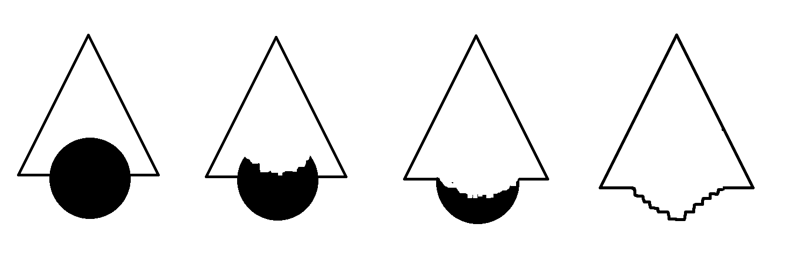
\includegraphics[width=0.94\linewidth]{order1.jpg}
	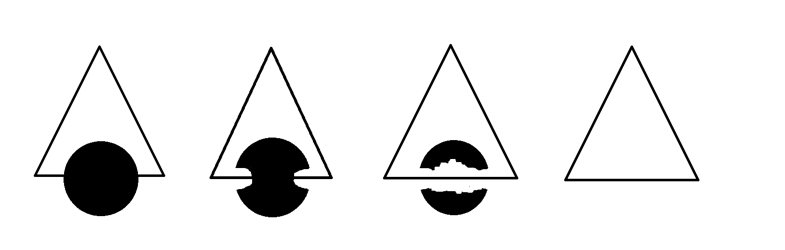
\includegraphics[width=1.0\linewidth]{order2.jpg}
	\caption{\textbf{The importance of the inpainting order}. The first group of images is the process of being inpainted from the up to the bottom, the second group of images is the process of being inpainted from the specific order.}
\end{figure}

In order to understand the importance of the inpainting order, a comparison between the specific order and fixed order is shown in Figure.1. the first group of images is using the up-to-bottom patch selection. Due to the target patch is always influenced by the nearby patch, so the bottom horizontal line of the triangle has not been inpainted. But if we do inpainting from the intersection of the target region and the bottom horizontal line, just as is shown in the second group of images. The horizontal line will be inpainted much better.

Therefore, a better image inpainting algorithm would be one that gives higher priority of synthesis to those regions of the target region which lie on
the continuation of image structures, as shown in the second group of Figure.1. 

\subsection{Our proposed method}
According to the two key observations mentioned above, the selection of patch that do inpainting first effects the final result much. So we should carefully select the specific patch. 
\begin{figure}
	\centering
	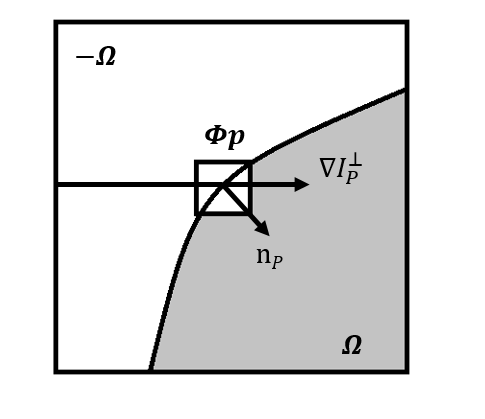
\includegraphics[width=0.94\linewidth]{region.jpg}
	\caption{\textbf{Notation figure}. The mask region and and the know region. The gradient and the unit vector is shown in the figure}
\end{figure}

Based on the image itself, in order to restore the original image, we should start from the intersection of the real line in image and the margin of the mask. So we use the dot cross result of the gradient and the unit vector orthogonal to the margin of the target region. Given a patch $\Phi_p$ centred at the point p for some $p \in \Omega$ (see Figure.2.), we define its priority $P(p)$ as the product of two terms:
\begin{equation*}
\centering
P(p)=C(p)*D(P)*E(p)
\nonumber
\end{equation*}

Where $C(p)$ is the confidence term of the patch $p$, $D(p)$ is the data term of the patch p, $E(p)$ is the evaluation term, which records the mask region in the target patch. 

Confidence term represents the amount of reliable information surrounding the pixel $p$. The
intention is to fill first those patches which have more of their pixels already inpainted, with additional preference given to pixels that were inpainted early on (or that were never part of the target region), it is calculated as follow:
\begin{equation*}
\centering
C(p)=\frac{\sum_{q\in \Phi _p\cap(-\Omega)}*C(q)}{|\Phi_p|}
\nonumber
\end{equation*}

Where $\Phi_p$ is the patch region, $|\Phi_p|$ is the area of the patch region. $\Omega$ is the target region, which is under the mask. $-\Omega$ is the region except for target region, it's the known region. During initialization, the confidence value is set to 1 in known region and 0 in mask region. 

Data term represents the real line or margin information in image. This factor is of
fundamental importance in our algorithm because it encourages linear structures to be synthesized first. It is the dot cross of the gradient and the unit vector orthogonal to the margin of the target region. It is calculated as follow:
\begin{equation*}
\centering
D(p)=\frac{|\nabla I^\bot_p \cdot n_p|}{\alpha}
\nonumber
\end{equation*}

Where $\nabla I^\bot_p$ is the gradient of image in pix $p$. $n_p$ is the unit vector orthogonal to the margin of the target region.

Evaluation term represents the weight of each pixel in the target patch, which records the area of mask region in the target patch. It is calculated as follow:
\begin{equation*}
\centering
E(p)=\frac{1}{\sum_{q \in \Phi_p \cap \Omega}q}
\nonumber
\end{equation*}

Where $\Phi_p$ is the patch region, $\Omega$ is the target region.

After defined the priority function of each patch, out algorithm work as the following steps.

First, given the input image and the input mask, initialize the whole patch in the margin with confidence term, data term and evaluation term. 

Next, compute the whole priority of each patch in mask margin, choose the maximum priority patch.

Then, traverse the patch that is near the target patch, compute the Euclidean distance of each pair of patch, find the exemplar patch minimizing the Euclidean distance.

Finally, copy the exemplar patch to the target patch where the pixel is unknown. And repeat these steps until there is no mask in the input image.

\subsection{Implementation details}
We implemented our algorithm in python. When we calculate the confidence term, data term and evaluation term, we used updated priority queue to operate data. It will save lots of time doing useless check and computing. 

We apply different size of patch and compare the result with each other. According to out experiment, patch size $3*3$ or $5*5$ will result in better result.

We assign normalization parameter $\alpha$ to 255 when we do inpainting. Due to the RGB form of our experiment images. It works well when assign any other significant value.

In all experiment, the size of mask was set to be larger than the patch size. And the image size is equal or larger than twice the mask size. Mask can be any shape.

We use a lot of images to test our algorithm, it may need much time when the mask is large, but it can successful handle different size of mask. Which is better than previous field of expert model \cite{ijcv09}, which will result in smoothing and blurring when mask size is large.
